\section{Frequency mode 02}
\label{FM02}

\subsection{Spectra}
\label{FM02:spectra}

\begin{figure}[ht]
    \centering
    \begin{subfigure}[b]{0.9545\textwidth}
        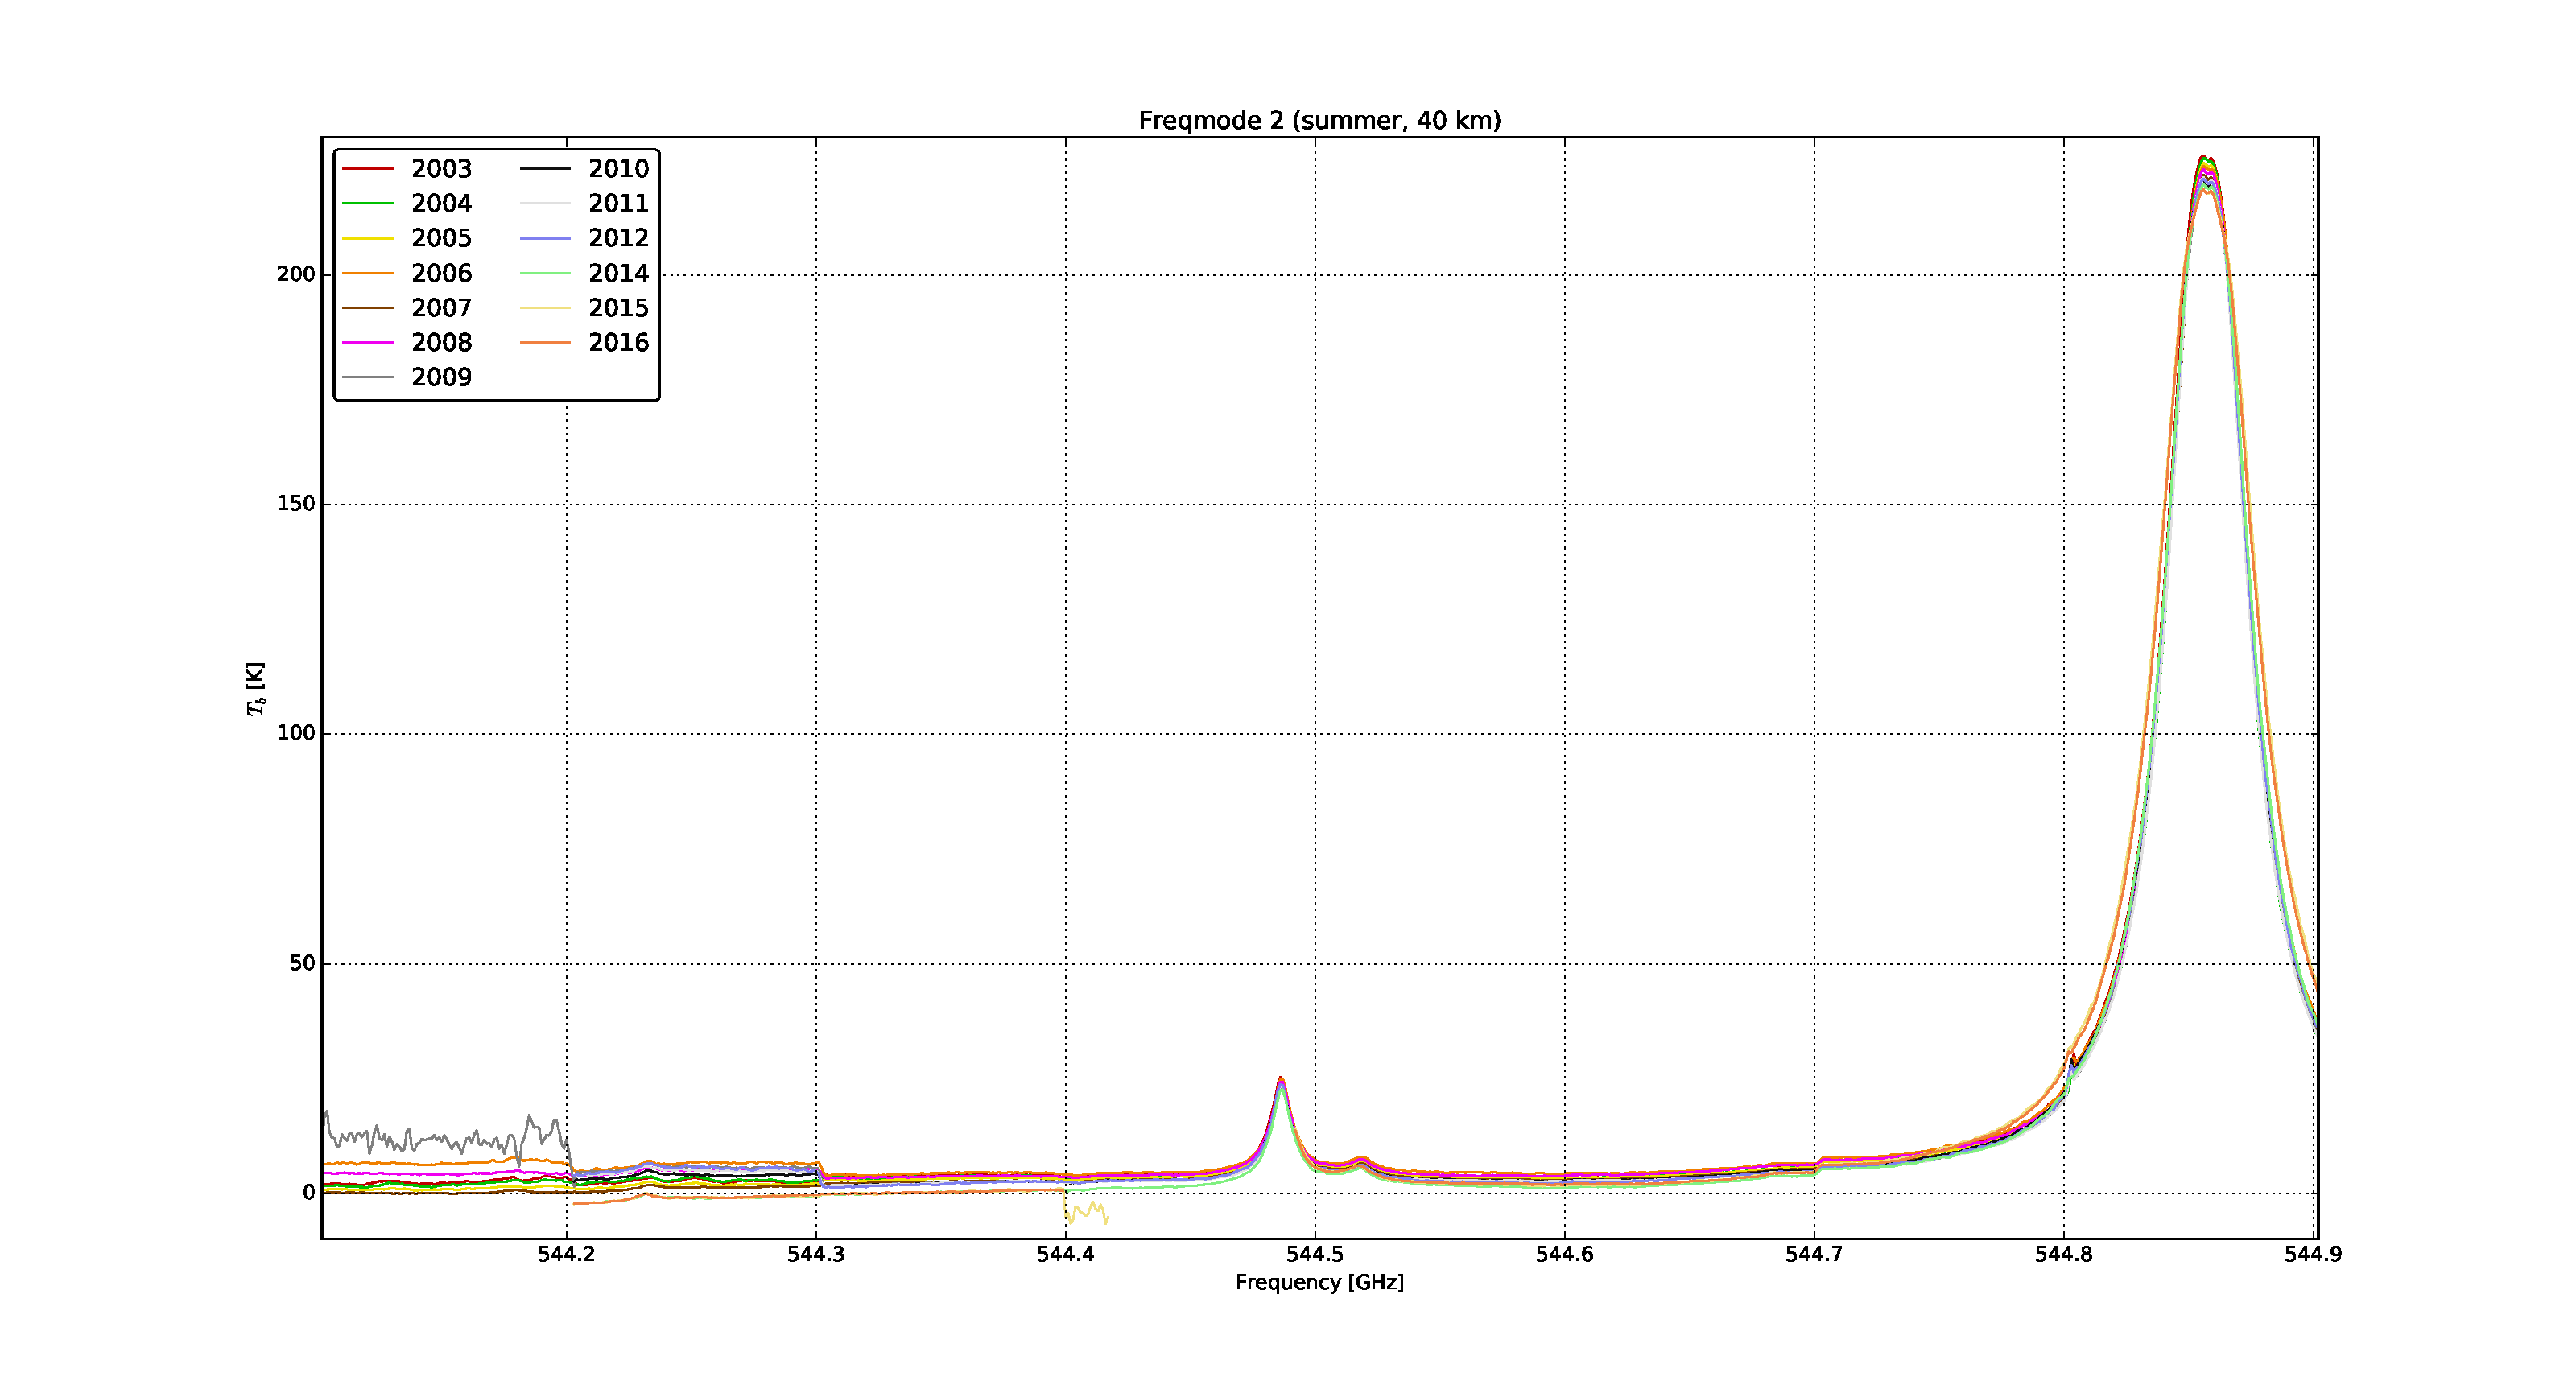
\includegraphics[width=\textwidth]{fm_02_spectra_summer}
        \caption{summer; 2014--2016 from FM~102}\label{fig:spectra:02:summer}
    \end{subfigure}
    \begin{subfigure}[b]{0.9545\textwidth}
        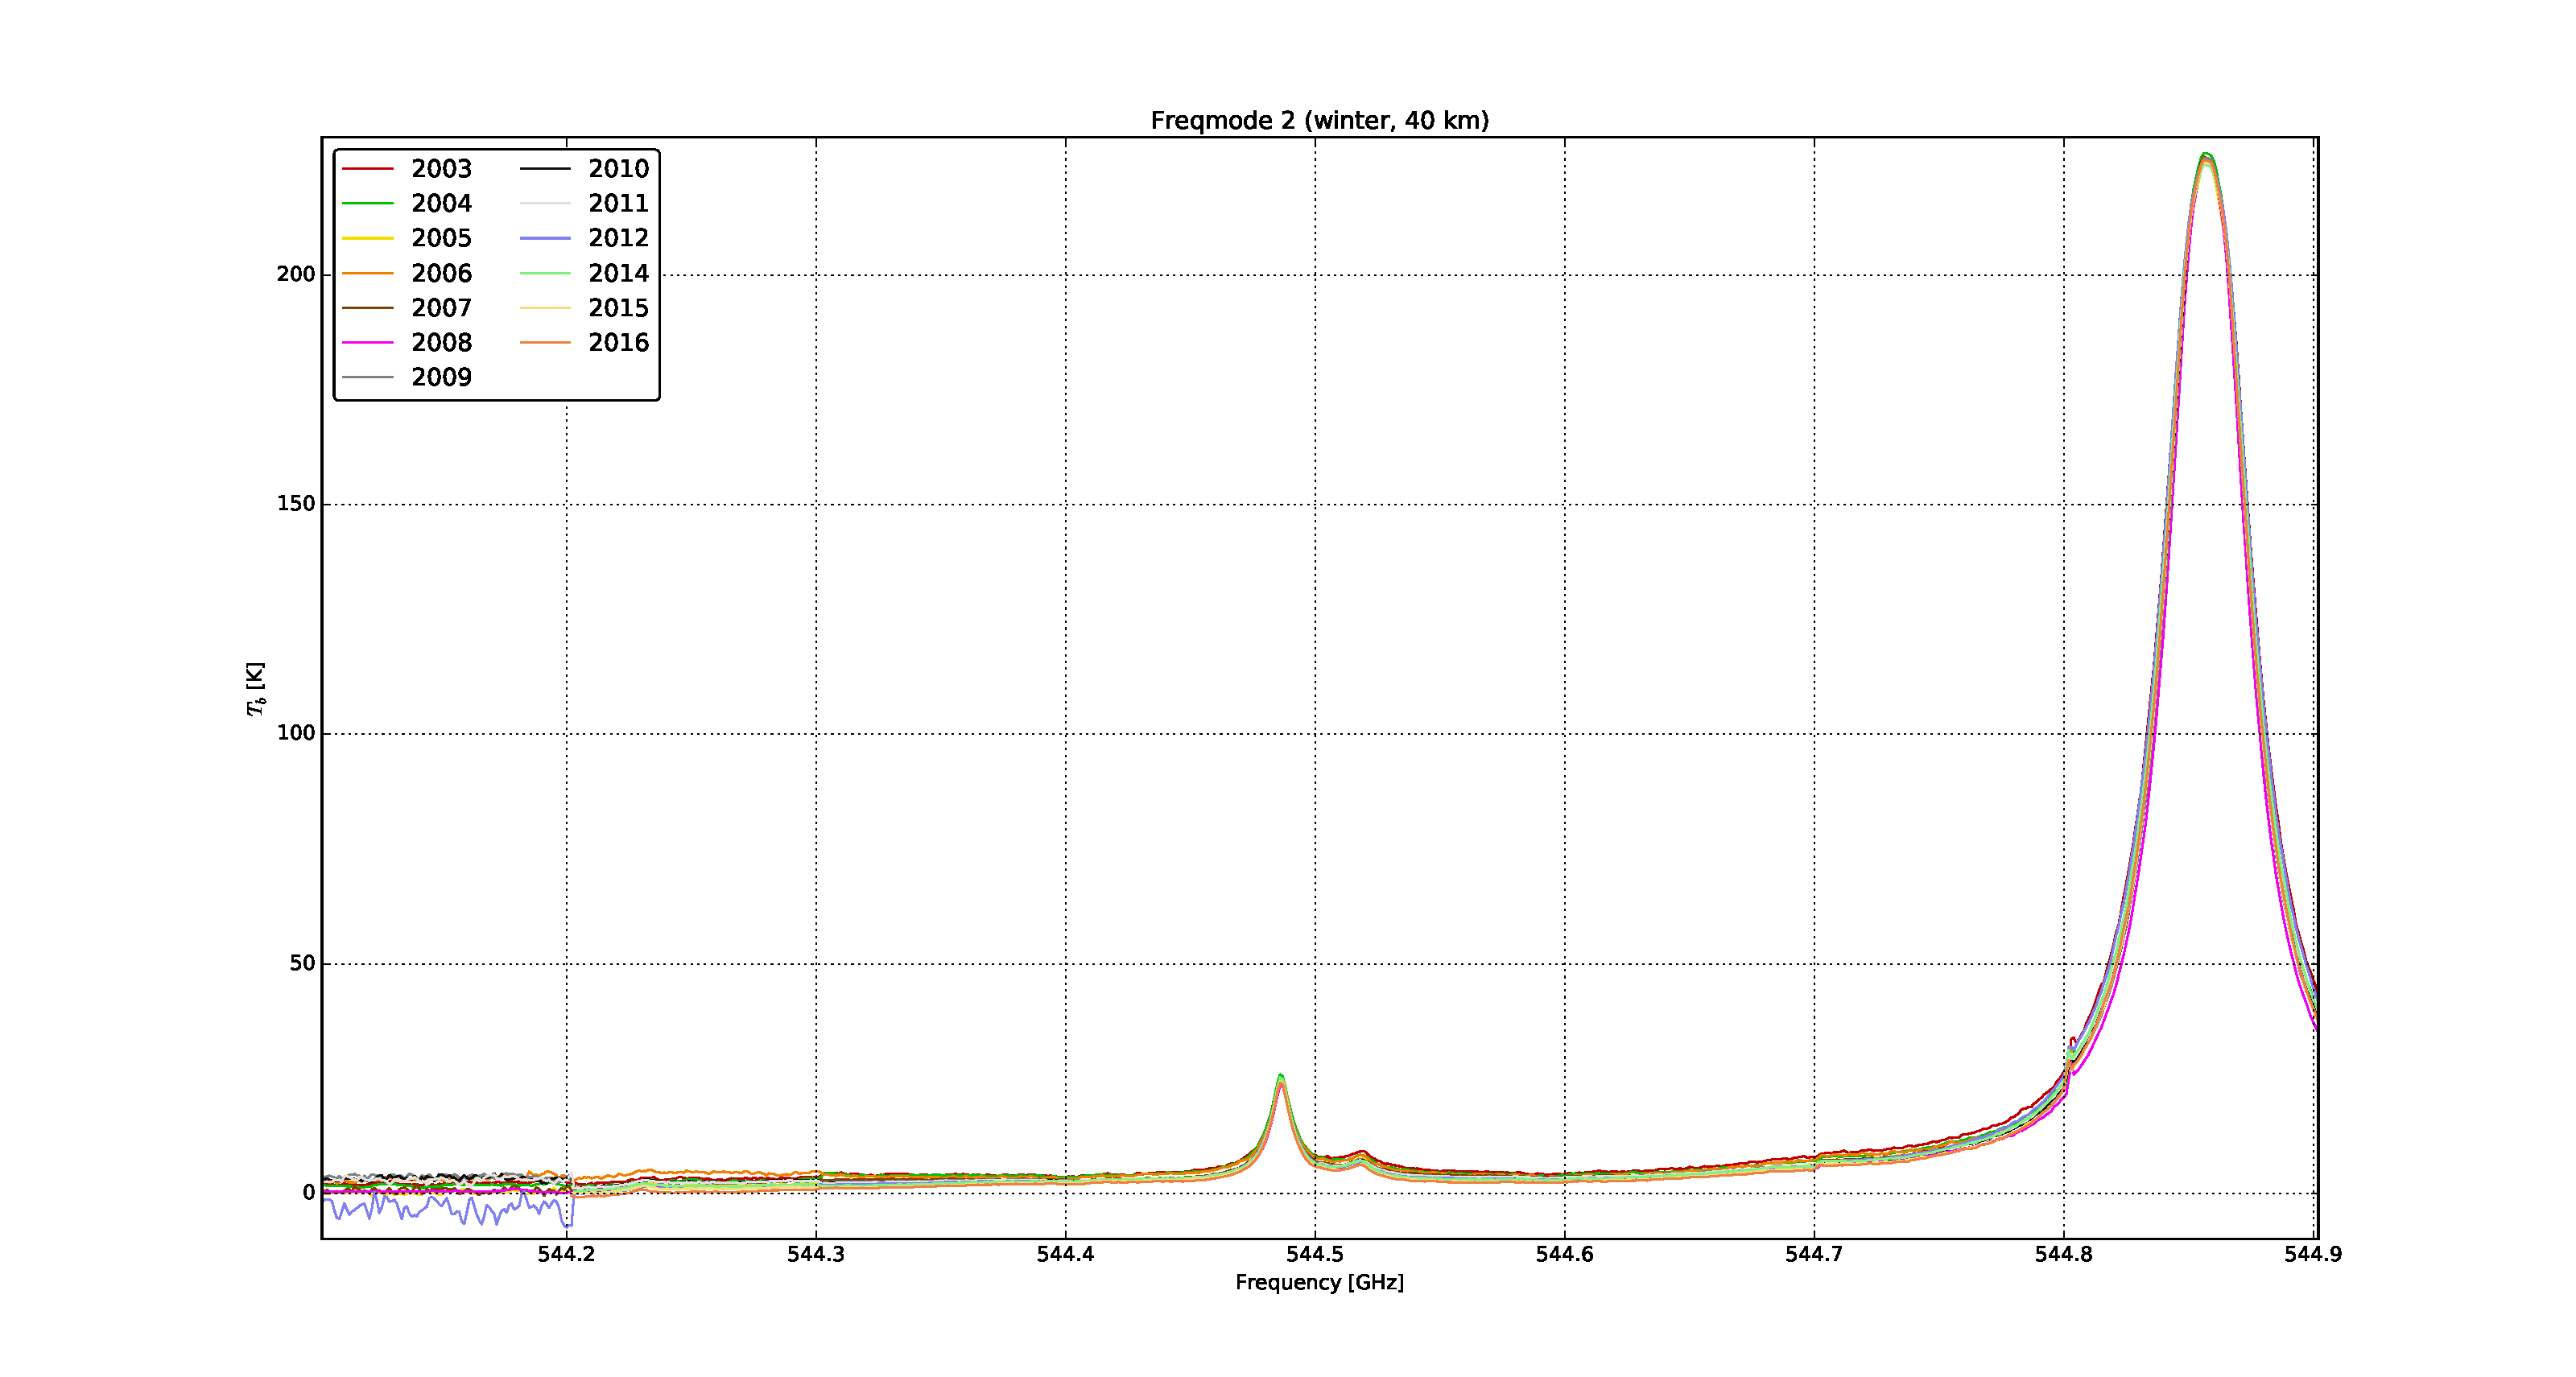
\includegraphics[width=\textwidth]{fm_02_spectra_winter}
        \caption{winter}\label{fig:spectra:02:winter}
    \end{subfigure}
    \caption{Annual median spectra for FM~02 for altitude interval 35--45~km at
        equatorial latitudes. The unhealthy sub-bands 1 and 2 to the left of
        $\sim544.3\,\mathrm{GHz}$.
        }\label{fig:spectra:02}
\end{figure}

\begin{figure}[ht]
    \centering
    \begin{subfigure}[b]{0.9545\textwidth}
        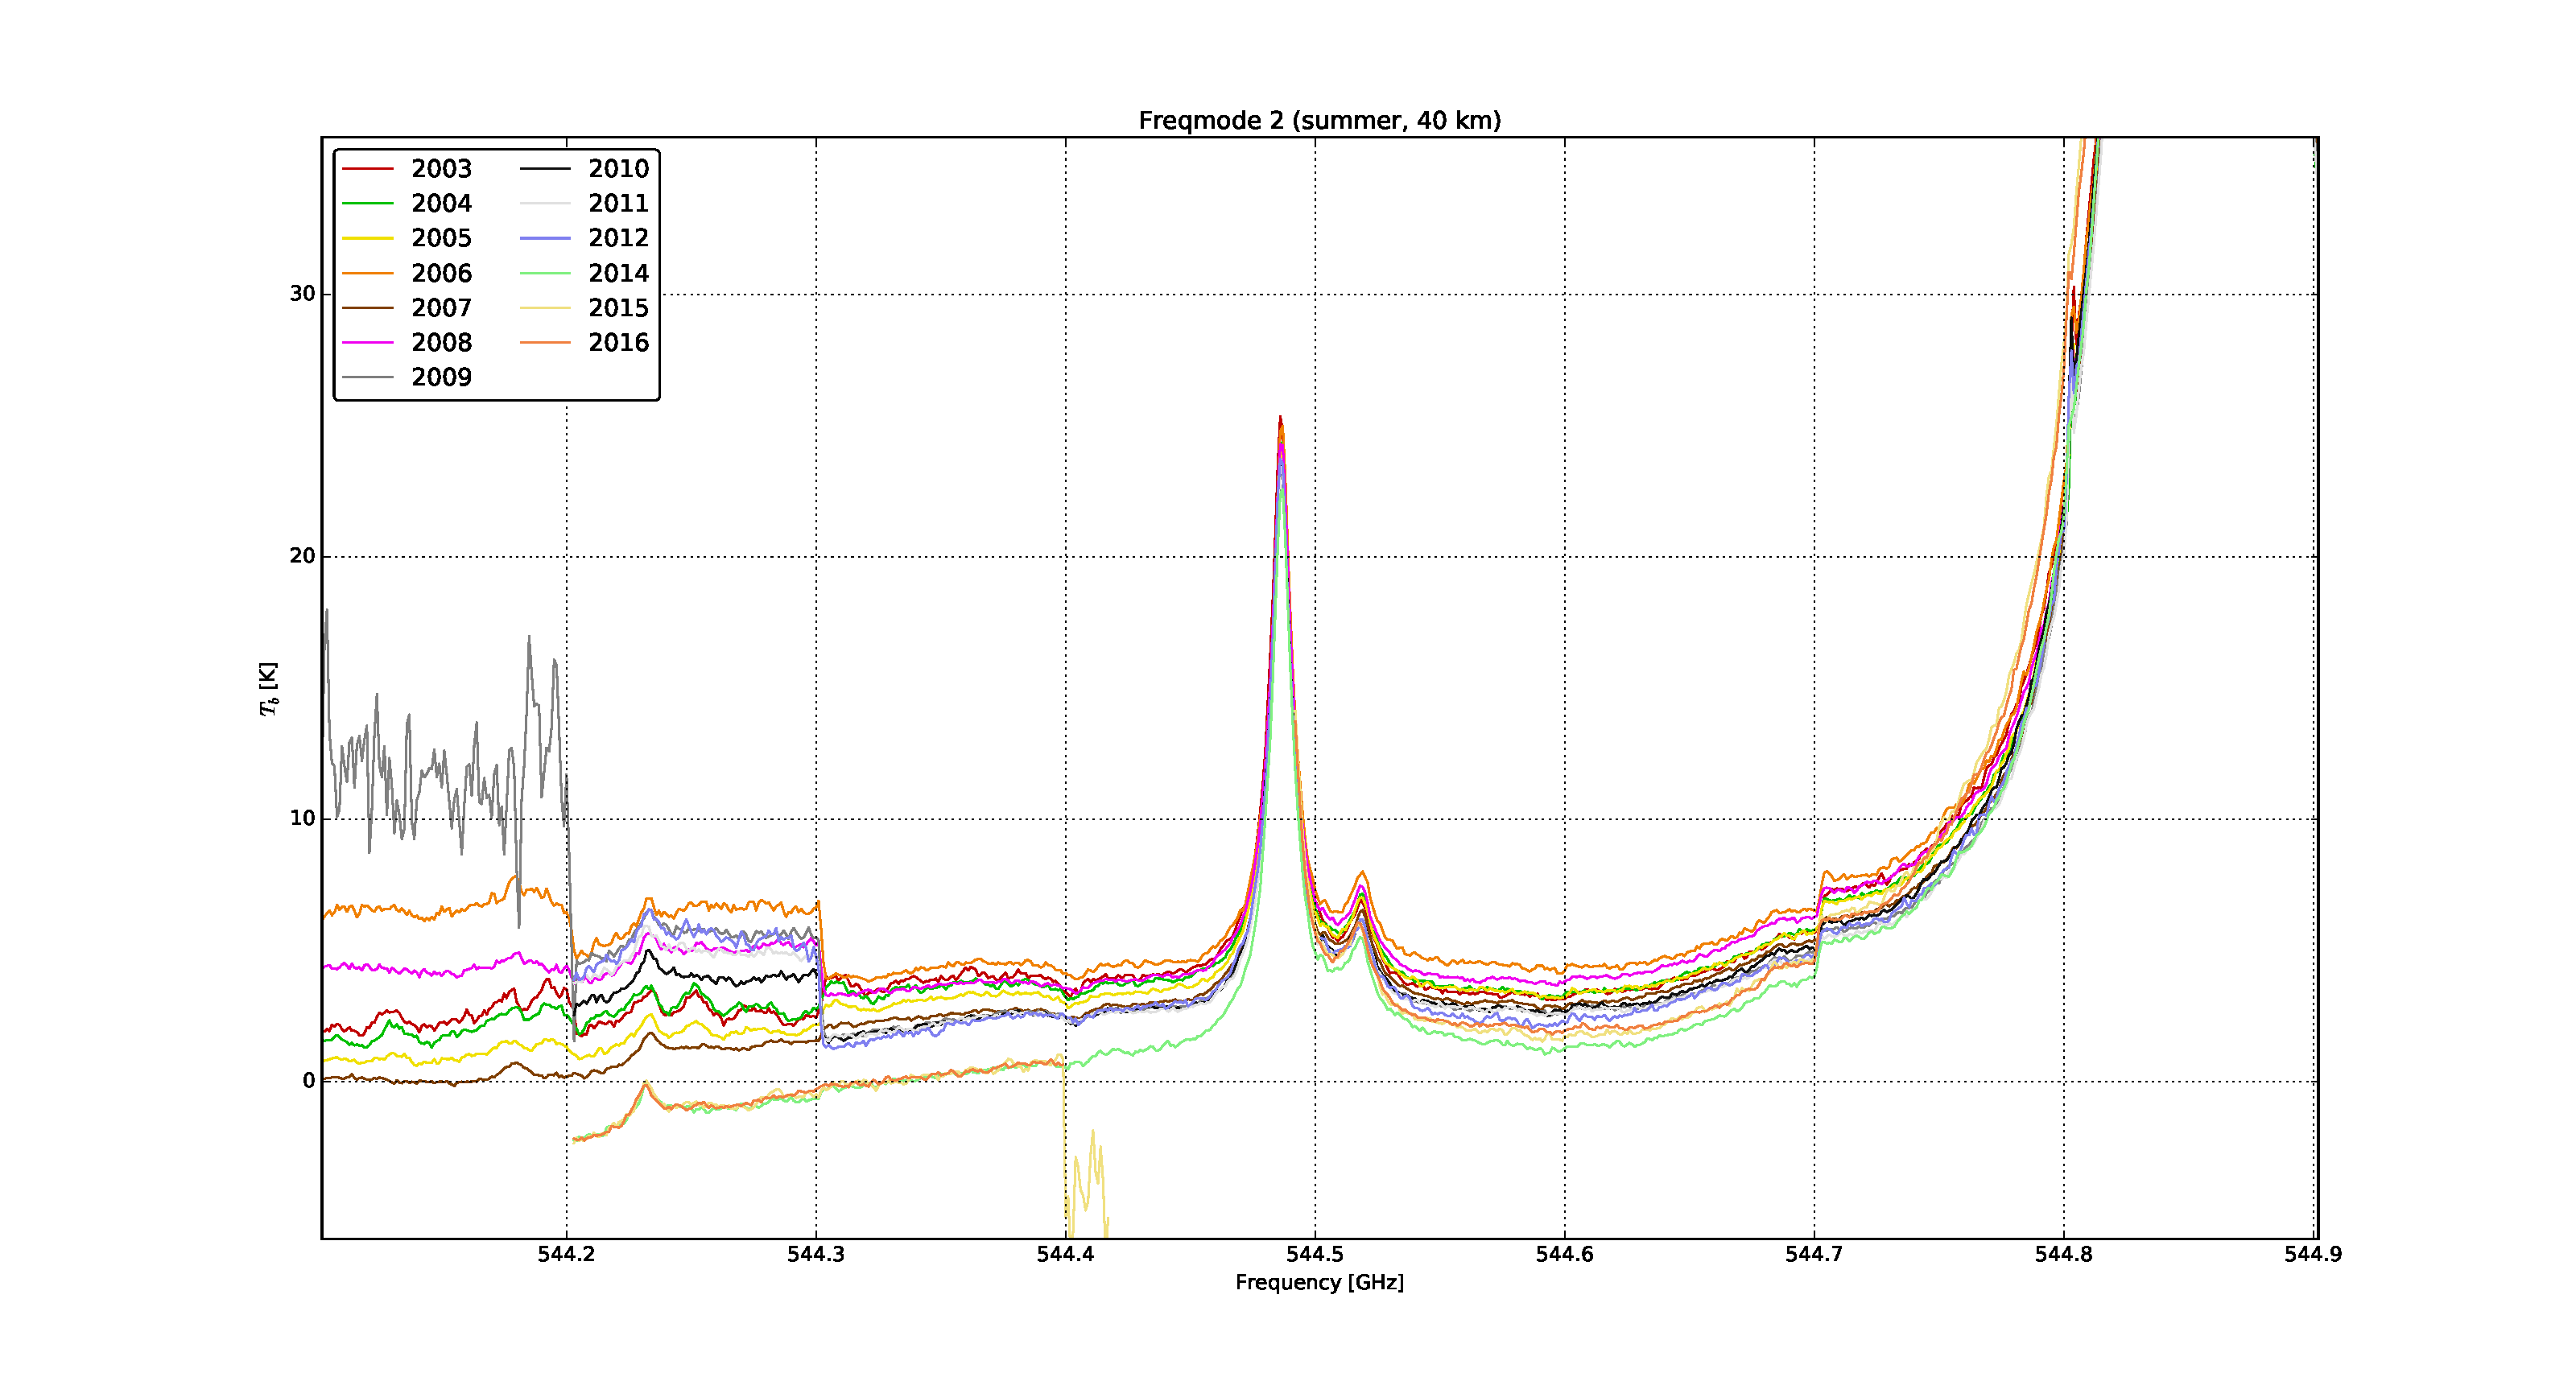
\includegraphics[width=\textwidth]{fm_02_spectra_summer_zoom}
        \caption{summer; 2014--2016 from
            FM~102}\label{fig:spectra:02:summer:closeup}
    \end{subfigure}
    \begin{subfigure}[b]{0.9545\textwidth}
        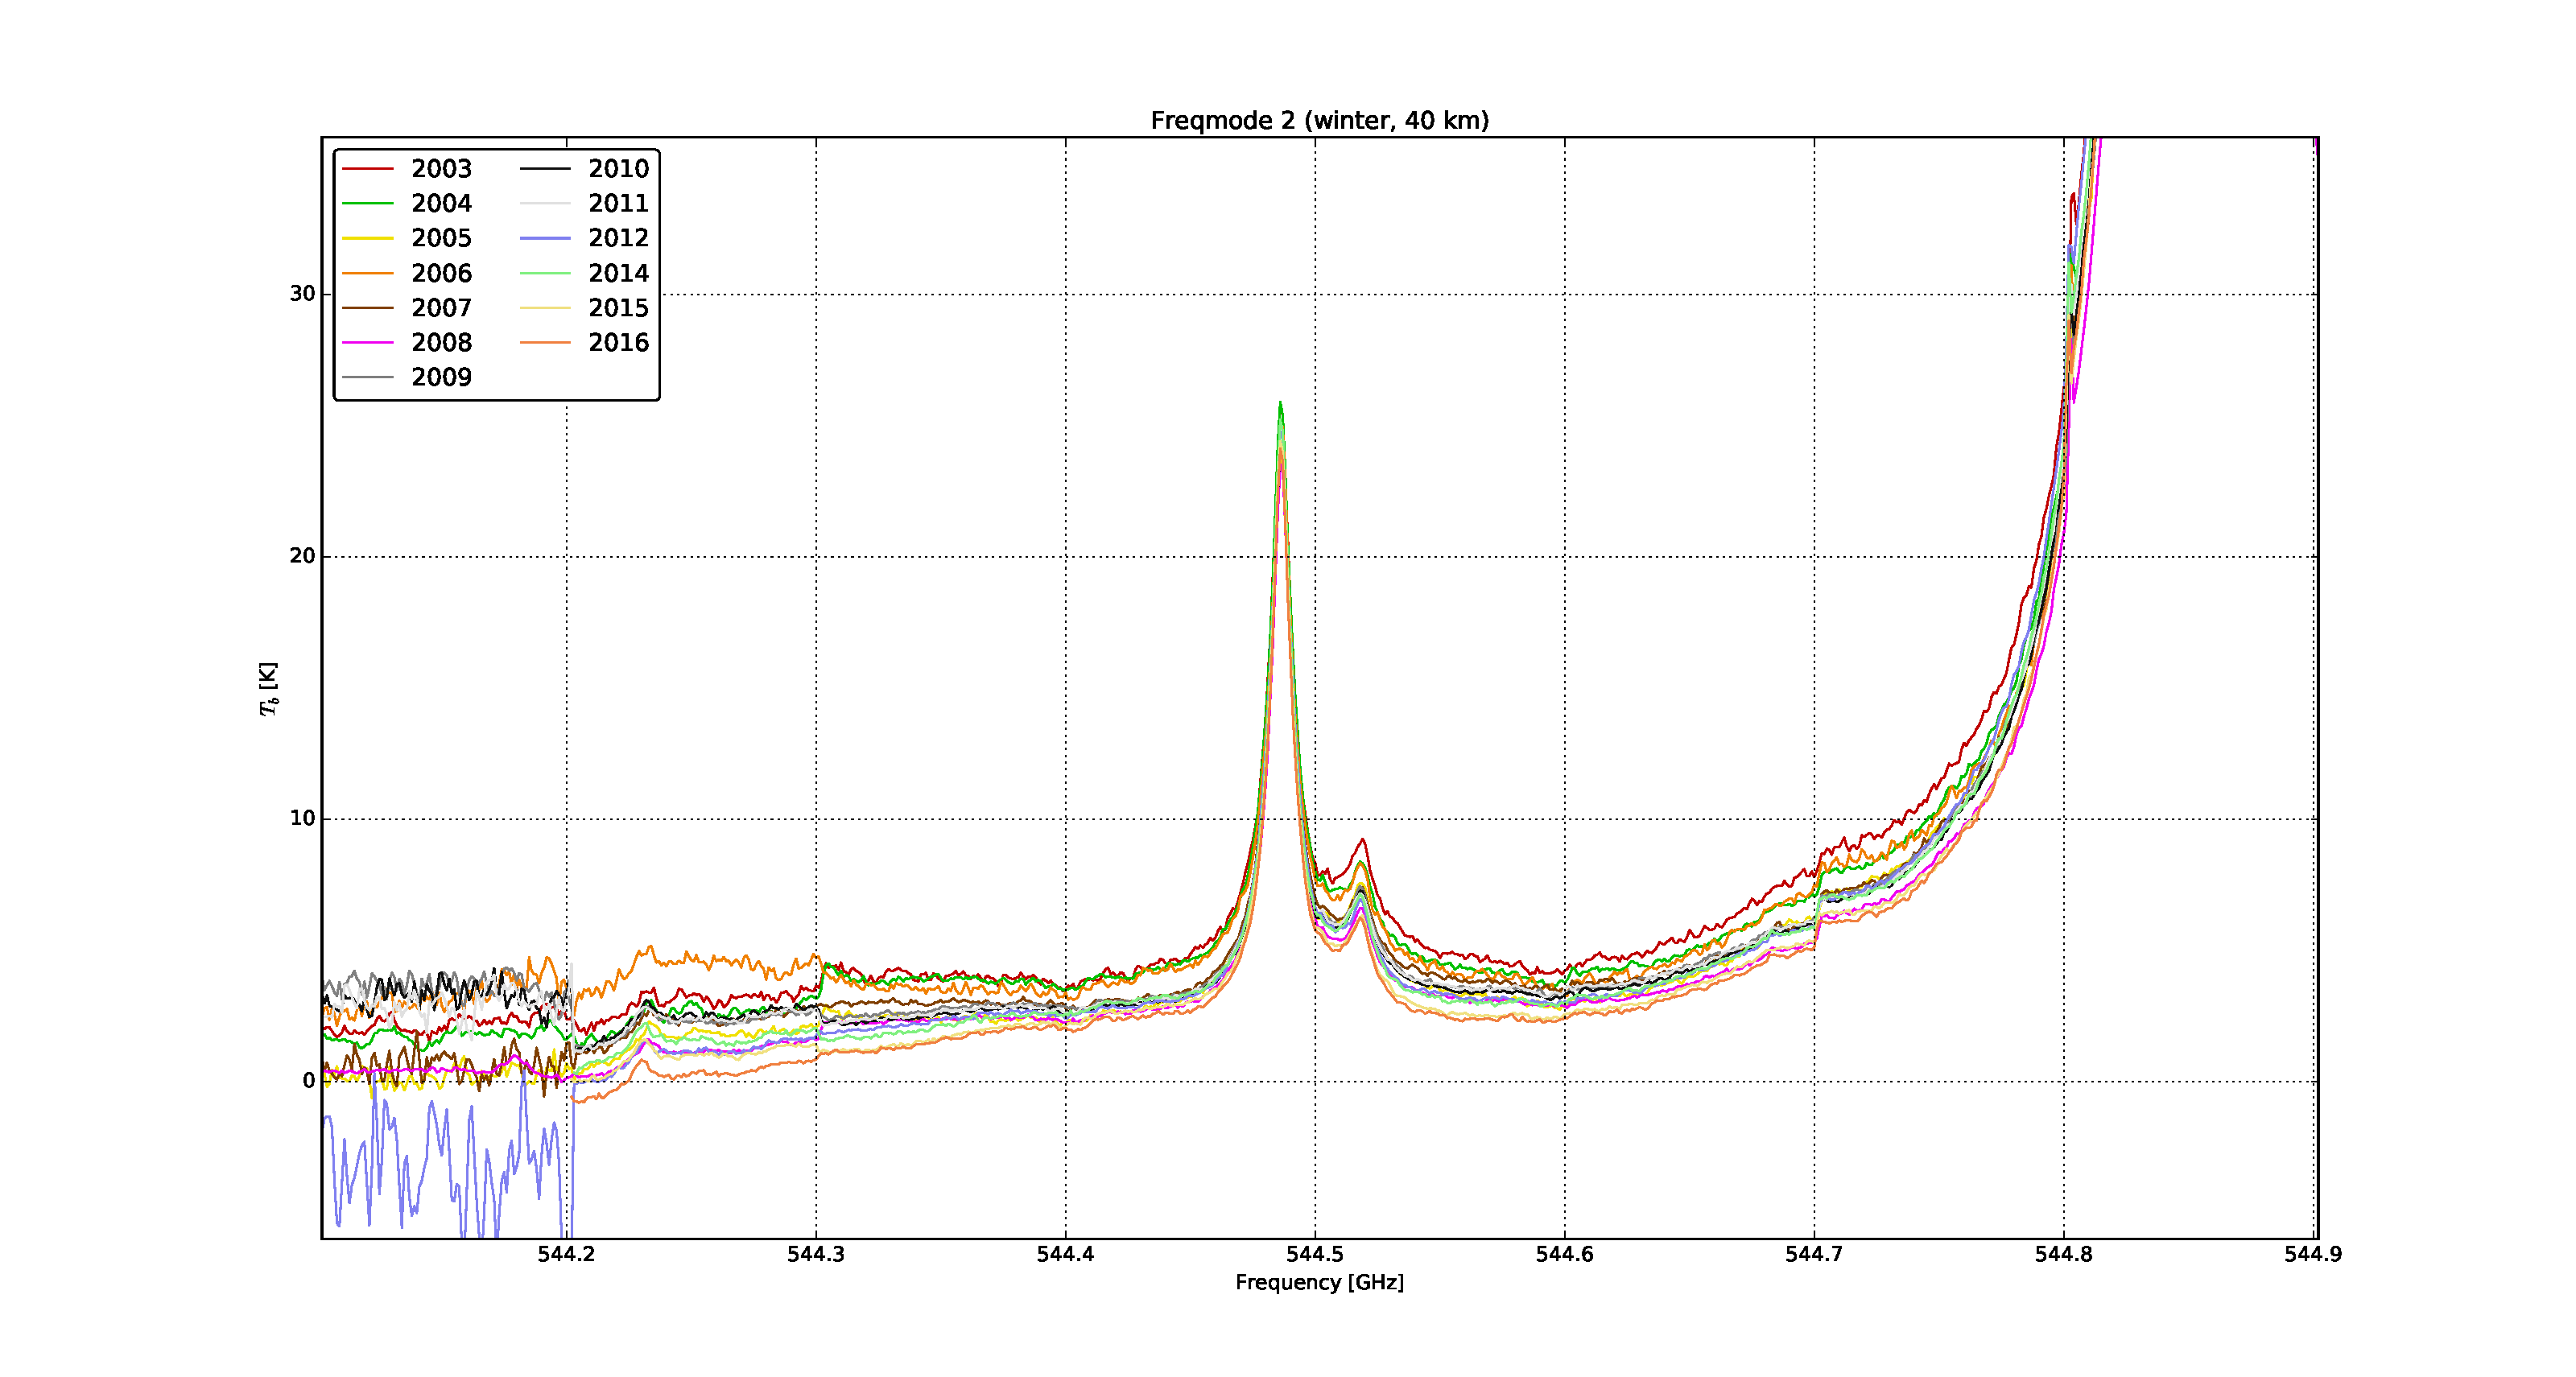
\includegraphics[width=\textwidth]{fm_02_spectra_winter_zoom}
        \caption{winter}\label{fig:spectra:02:winter:closeup}
    \end{subfigure}
    \caption{Close-up of the annual median spectra for FM~02 for altitude
        interval 35--45~km at equatorial latitudes.  The unhealthy sub-bands
        1 and 2 are to the left of $\sim544.3\,\mathrm{GHz}$.
        }\label{fig:spectra:02:closeup}
\end{figure}

\noindent
Yearly median spectra for summer and winter at $\sim40\,\mathrm{km}$ are shown
in Fig.~\ref{fig:spectra:02}.  These and the close-ups seen in
Fig.~\ref{fig:spectra:02:closeup} show that the spectra seem to fall in two
categories, depending on whether they were obtained before or after 2009, with
spectra obtained during later years being clustered a lower baseline
temperature.  This is examined in more detail in Sec.~\ref{FM02:baseline}
below.


\subsubsection{Jumps}
\label{FM02:jumps}
As can bee seen around $544.7$ and $544.8\,\mathrm{GHz}$ there are jumps in
spectra.  These occur between sub-bands and due to mismatches when the data
from the different sub-bands is combined.  Unfortunately, it is not a simple
shift, i.e.\ the jump at $544.7\,\mathrm{GHz}$ is not the same as that at
$544.8\,\mathrm{GHz}$.  These mismatches need to be compensated for either
during the Level~2 processing or, ideally, at an earlier stage.


\subsection{Sideband leakage}
\label{FM02:sbl}
The structure of the spectra of FM~2 is such that the sideband peaks often
overlap with the main peaks, and the sideband peaks that are distinct are
unfortunately localised in sub-bands of bad quality.  It is therefore difficult
to draw any definite conclusions regarding the long term tendency of the
sideband leakage for this mode.  However, the estimated sideband leakage seems
to be confined to 3--5\% (or more conservatively to 2--6\%), with no clear
tendency to either increase or decrease over time.  The overall decrease in the
\chem{OO^{18}O} peak and basline seen in Fig.~\ref{fig:peaks:21} could
ostensibly both be due in part to a decrease in the sideband leakage, but this
is mere speculation.


\subsection{Seasonality}
\label{FM02:seasonality}

\begin{figure}[ht]
    \centering
    \begin{subfigure}[b]{0.9545\textwidth}
        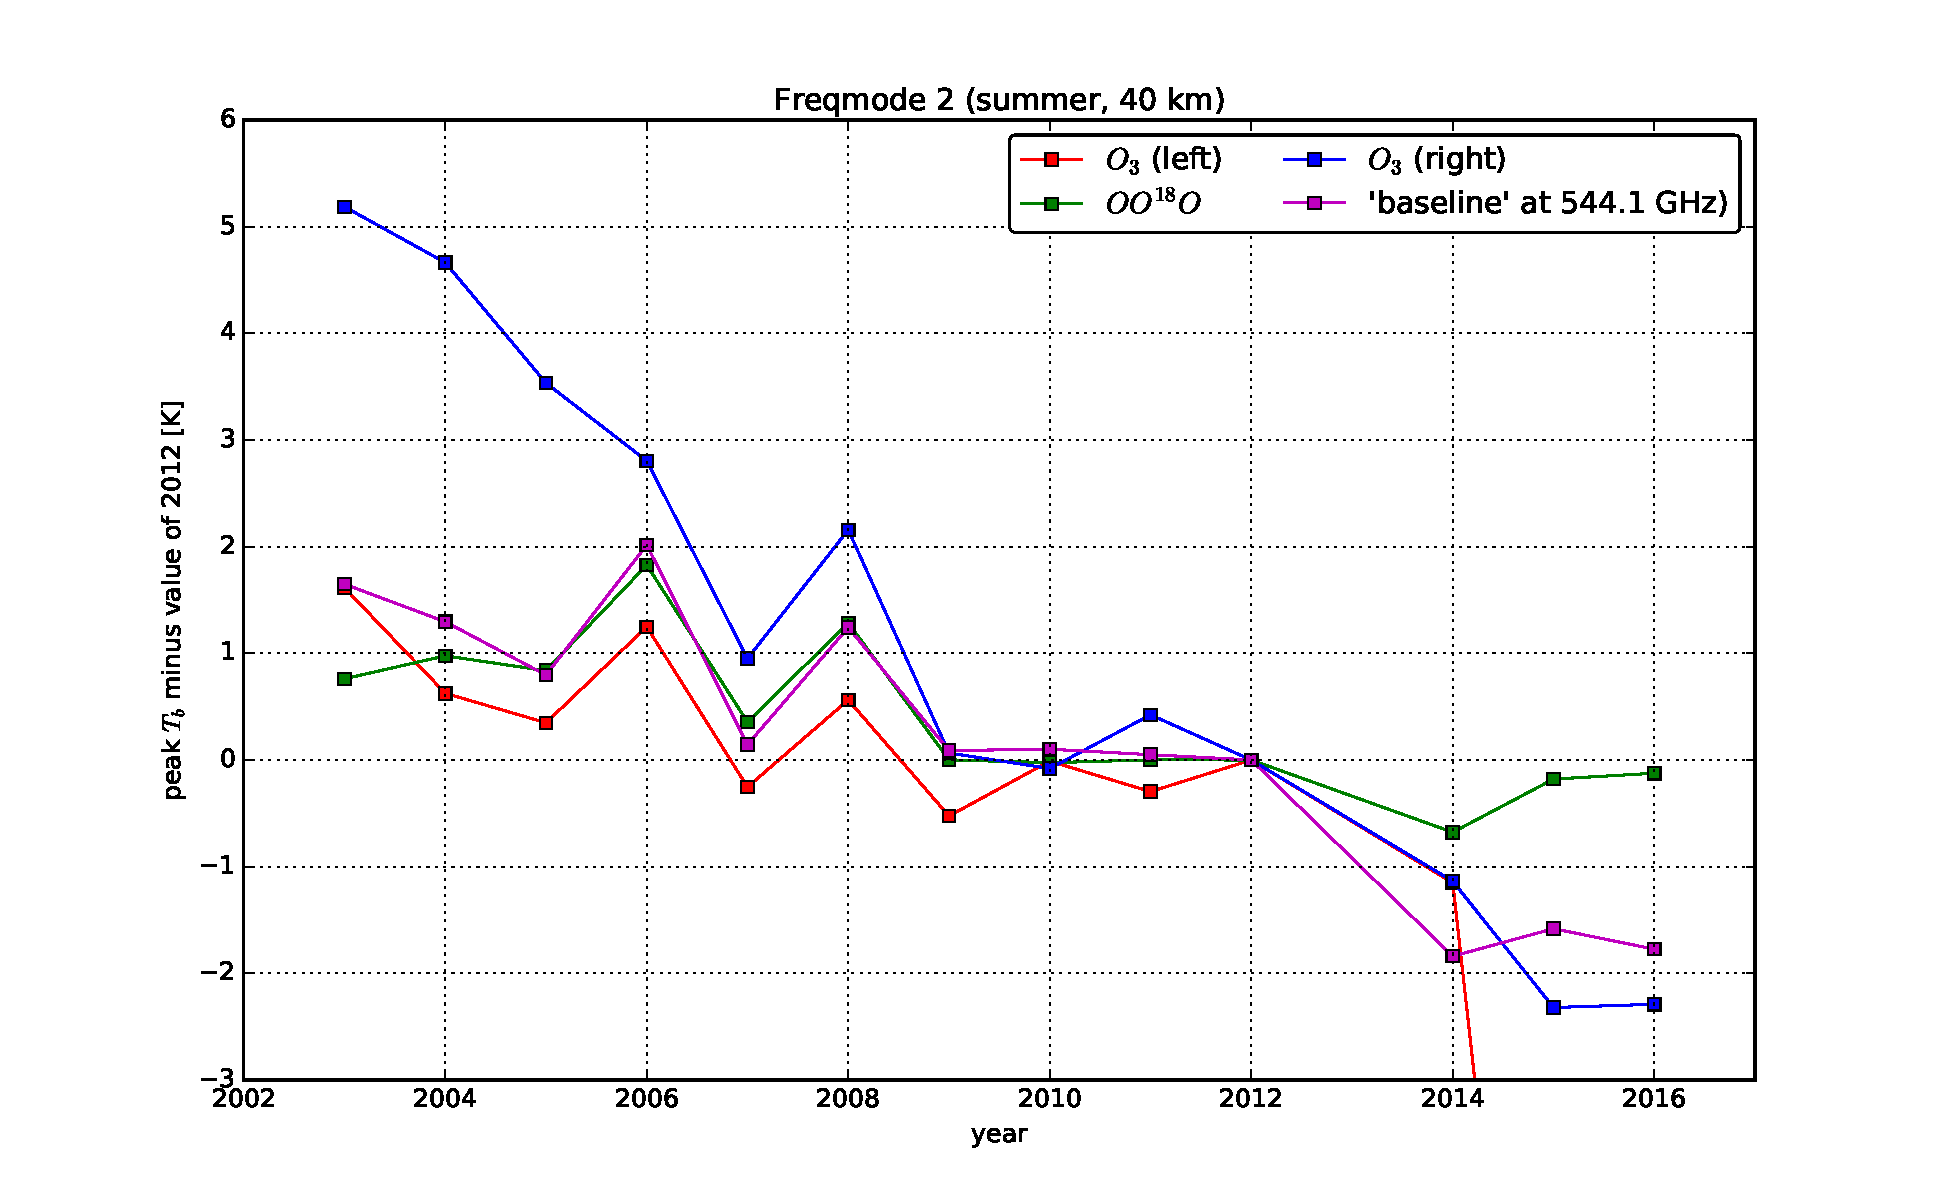
\includegraphics[width=\textwidth]{fm_02_peaks_summer_debias}
        \caption{summer; 2014--2016 from FM~102}\label{fig:peaks:02:summer}
    \end{subfigure}
    \begin{subfigure}[b]{0.9545\textwidth}
        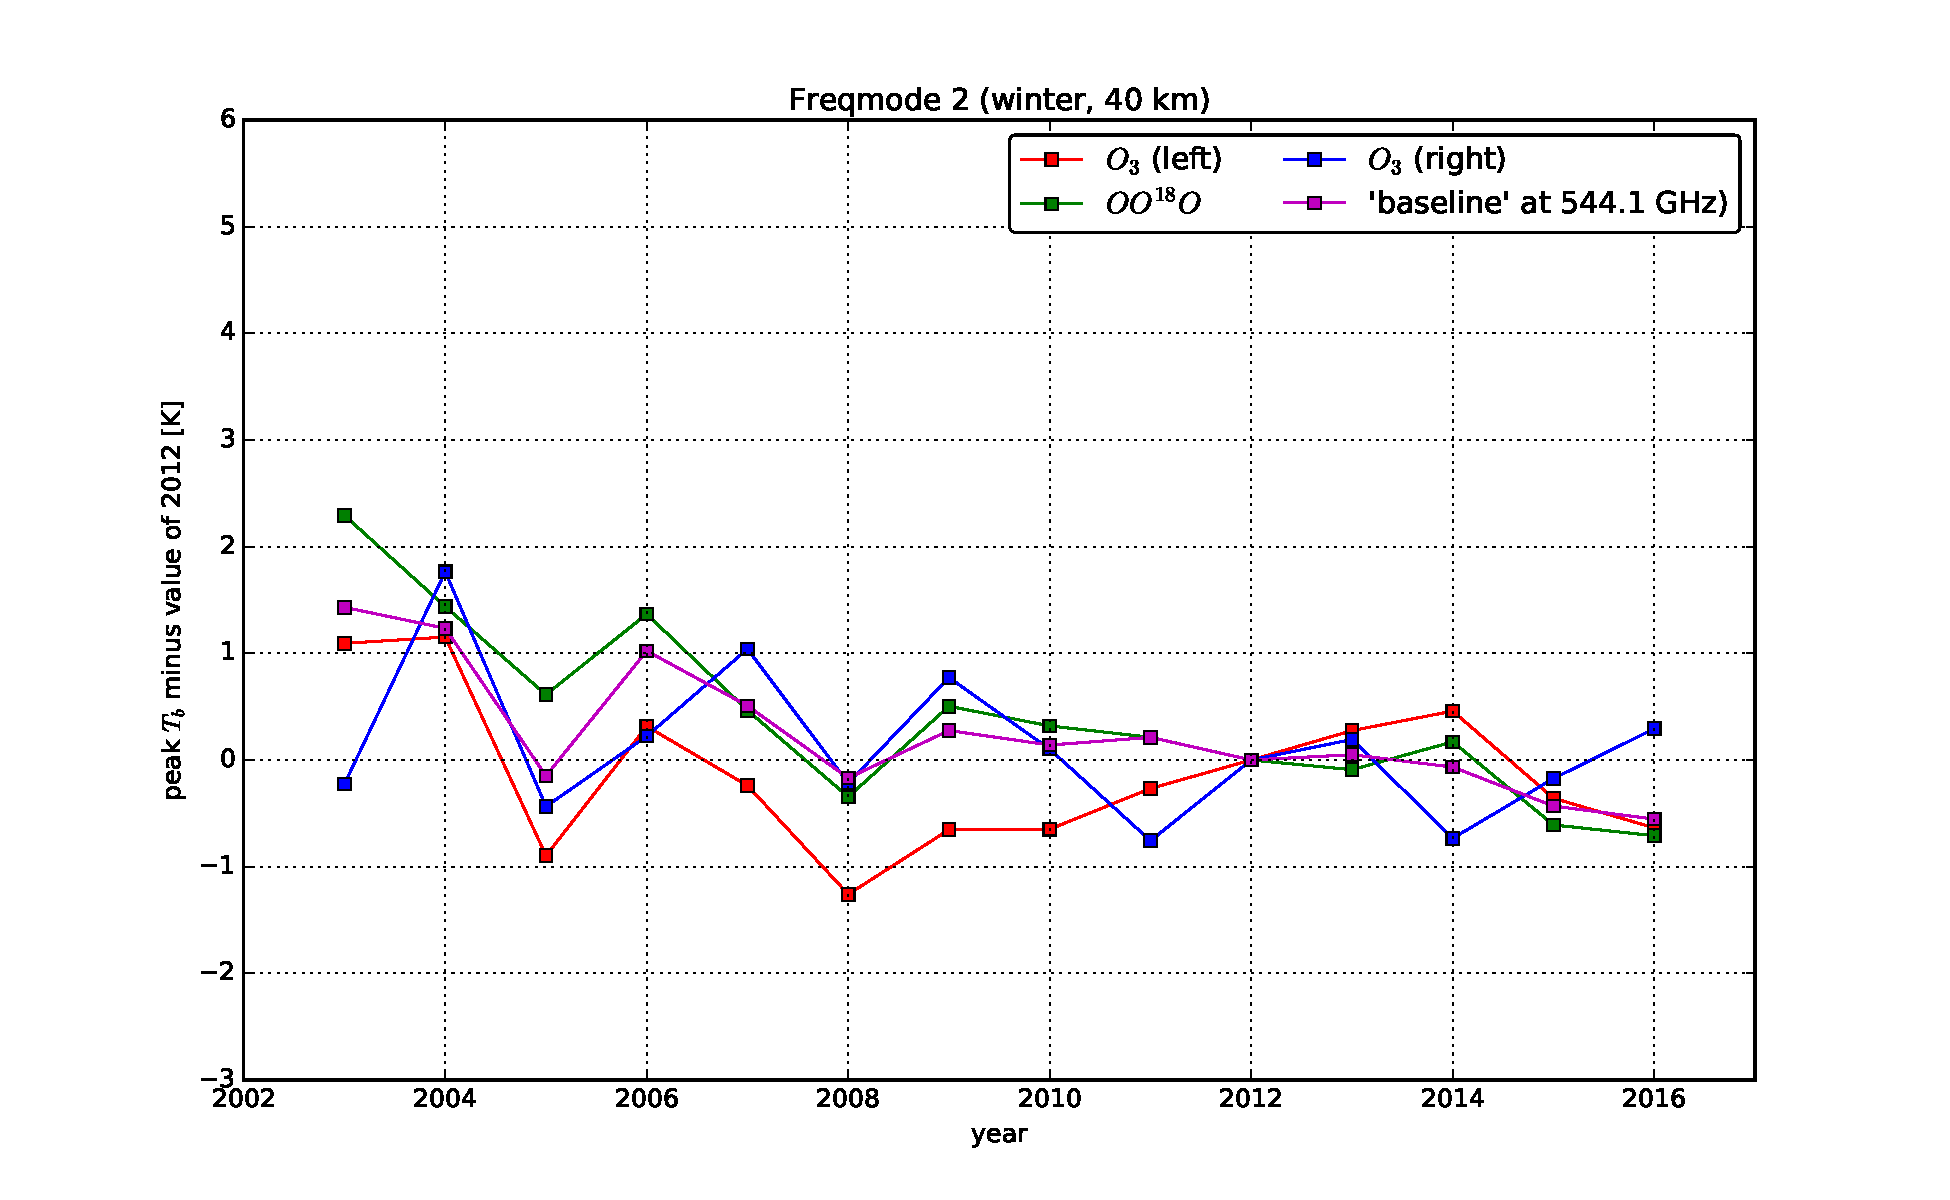
\includegraphics[width=\textwidth]{fm_02_peaks_winter_debias}
        \caption{winter}\label{fig:peaks:02:winter}
    \end{subfigure}
    \caption{Difference of annual median peak values and their respective
        values for 2012 for FM~02 for altitude interval 35--45~km at
        equatorial latitudes. Values extracted for the left \chem{O_3} peak
        at~$\sim544.48\,\mathrm{GHz}$, the \chem{OO^{18}O} peak
        at~$\sim544.52\,\mathrm{GHz}$, and the right \chem{O_3} peak
        at~$\sim544.86\,\mathrm{GHz}$, in Fig.~\ref{fig:spectra:02}.  A
        ``baseline'' value was also estimated
        at~$\sim544.10\,\mathrm{GHz}$.  The unhealthy sub-bands 1 and 2 are to
        the left of $\sim544.3\,\mathrm{GHz}$.
        }\label{fig:peaks:02}
\end{figure}

\noindent
Fig.~\ref{fig:peaks:02:summer} shows that the large \chem{O_3} peak
at~$\sim544.86\,\mathrm{GHz}$ was steadily decreasing during the summers up to
2009, whereafter it appears to have stabilised (n.b.~the values for 2014--2016
are from FM~102 and are therefore not directly comparable).  This may be due to
normal atmospheric variations, such as those due to the solar cycle, but no
similar trend is as clearly evident in the other two peaks, which appear to
follow the change in baseline.  Since the peak at~$\sim544.86\,\mathrm{GHz}$
has a very high intensity, at least part of the change in the baseline is
likely due to the changes in this peak value.

In contrast to the trend seen for the summers, Fig.~\ref{fig:peaks:02:winter}
shows no clear downward trend for the right-most peak, whereas the left-most
\chem{O_3} peaks appears to follow the baseline trend up to 2009, after which
it shows a slight increase in spite of a continually falling baseline.


\subsection{Change of ``baseline'' for later years}
\label{FM02:baseline}
As noted in Sec.~\ref{FM02:spectra} above, the baseline of the spectra appears
to have decreased over the years. Looking at the values around
$544.1\,\mathrm{GHz}$ in Fig.~\ref{fig:spectra:02:closeup}, the values after
2009 are all clustered arour $3\,\mathrm{K}$.  In contrast, the corresponding
values for the earlier years, though showing a higher variation, have been
decreasing from $4$--$5\,\mathrm{K}$ to the present levels.  This is the case
both for the (cold) summers and (warm) winters, though looking at
Fig.~\ref{fig:peaks:02:winter} the baseline appears to be decreasing again
after 2013 (a similar conclusion cannot be draw for the summer, since the
summer values for 2014--2016 are from FM~102 and are therefore not directly
comparable).

Further, it is worth noting that the baseline to the left of the central peak
appears to have aquired more of a slope during the later years of the mission,
as seen in Fig.~\ref{fig:spectra:02:closeup} (again, the data for 2014--2016
are from FM~102 and, though they show a similar tendency, are not directly
comparable).
